


\chapter{Application of Monte Carlo Sampling to Calculate Quantum Binding Free Energies from DFT Total Energies}


\section{Introduction}

The previous chapter showed that the classical and quantum potential energy surfaces do not match.  Woods et al. \cite{mullholland_qmmm} describe a method that applies an acceptance test to decide if the classically generated structure would fit into a desired potential, in this case QM/MM.  Within this chapter we will also accept to a QM/MM ensemble, but this will only be used a step toward a full QM ensemble.  This transition will be performed by using the Zwanzig equation (equation \ref{eq:Zwanzig}).  However, this makes the approximation that the QM/MM potential energy surface is parallel to the QM potential energy surface.  This stepwise method is possible because free energy is a state function, similar to the extended thermodynamic cycle as described previously.

\begin{center}
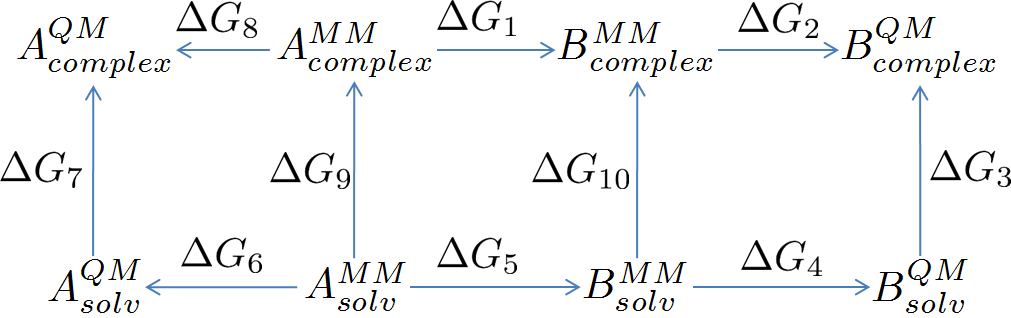
\includegraphics[width=15cm]{extended_thermodynamic_cycle.png}
 \captionof{figure}{Extended Thermodynamic Cycle}\label{fig:extended_thermodynamic_cycle}
\end{center}

The QM/MM calculations are much faster than the QM calculations, so with the approximation described above in place, a good representation of the QM ensemble should be built up quickly.

\begin{equation} \label{eq:Zwanzig}
\ \Delta G= -k_B T \ln \left\langle \exp \left[ -\beta \Delta U_{QM-MM} \right] \right\rangle_{MM} \\.
\end{equation}

%Finding a relatively computationally inexpensive method that can calculate accurate free energies of binding for large systems is one of the main challenges within computational chemistry.  Typically for large biologically relevant systems force fields are used, this is then highly dependent on the parameterisation used to describe the system.  The use of classical mechanics omits quantum only interactions, such as the exchange interactions, and cannot model any charge transfer or polarisation \cite{QM/MM_review}.  Ideally all conformational sampling would be performed using \textit{ab initio} molecular dynamics, but this is far too computationally expensive to be feasible.  Compromising chemical accuracy with speed leads to treating only part of the system (i.e. the binding pocket) within quantum mechanics and treating the rest with classical mechanics, QM/MM.  There are many applications of this method to calculate binding energies, however, there is a consistent problem when using this method if the QM region is chemically bound to the classical region.  This then involves cleaving these chemical bonds and capping them with appropriate functional groups.  QM/MM involves a large degree of expertise and setting up simulations for a non-expert can be highly nontrivial, it also neglects any long range quantum effects apparent in the system\cite{protein-ligand_interactions_book}.


%Another possibility is to use a guiding potential with a computational cost much lower than the desired potential.  This was first described by Warshel et al. \cite{Warshel_free_energy_correction} when he introduced the extended thermodynamic cycle.

%\begin{center}
%\includegraphics[width=15cm]%{extended_thermodynamic_cycle.png}
% \captionof{figure}{Extended Thermodynamic Cycle}%\label{fig:extended_thermodynamic_cycle}
%\end{center}


%This takes advantage of free energy being a state function and allows quantum corrections to classically obtained free energies.  This has been applied by sampling conformers using classical mechanics molecular dynamics, extracting regularly spaced uncorrelated snapshots, and perturbing to a more expensive potential such as QM/MM \cite{essex_qmmm} or fully quantum described system \cite{fox_mm_to_qm} using a single step free energy perturbation approach, making use of equation \ref{eq:Zwanzig}, the Zwanzig equation \cite{zwanzig}.  The fully quantum description of the entire system would be extremely costly using traditional cubic scaling DFT, but by using a linear scaling DFT such as ONETEP \cite{ONETEP} this computational cost is manageable.

%\begin{equation} \label{eq:Zwanzig}
%\ \Delta G= -k_B T \ln \left\langle %\exp \left[ -\beta \Delta U_{QM-MM} %\right] \right\rangle_{MM} \\.
%\end{equation}
%
%Where $k_B$ is the Boltzmann constant, $T$ is the temperature, $\Delta U_{QM-MM}$ is the potential energy difference between the desired potential (in this case QM) and the sampling potential (in this case MM), $\beta$ is $1/k_B T$, the $\langle \cdots \rangle$ represents an ensemble average and the subscript $MM$ represents the potential used to obtain the structures.

%In both references previously mentioned that apply this method \cite{essex_qmmm}\cite{fox_mm_to_qm}, the interaction energies of the systems are used.  Interaction energies are described simply by:

%\begin{equation}
%\ U_{interaction}=U_{complex}-U_{ligand}-U_{host} \\.
%\end{equation}

%This cancels out any intramolecular terms and any intermolecular interactions within the host.  The $complex$ is the entire system e.g. a ligand bound to a protein and in the same example $host$ would be the protein in the same geometry without the ligand present.  This makes the approximation that the conformation of the protein would be sampled in the absence of the ligand, additionally the Zwanzig equation has not been derived for use with interaction energies, but with total energies.  However, the use of total energies causes additional issues, one such minor issue is the calculation of the exponential of the large size difference between the quantum and classical system.  This can be overcome by using numerical tricks \cite{Berg_maths}.  Using the methods described by Fox et al. \cite{fox_mm_to_qm} makes the assumption that the configurational space sampled by the force field is parallel to the configurational space of the quantum potential.  

%When using total energies within this method, the assumption does not hold.  Unpublished results obtained by the author show an inexact overlap of conformational space, which leads to low energy outliers within the energy difference distribution.  These low energy snapshots then dominate the free energy obtained from equation \ref{eq:Zwanzig}, due to the calculation of the the exponential of the negative energy.  When this free energy is plotted as a function of the number of snapshots included, the graph shows ``sawtooth'' behaviour, which is typical of sampling issues \cite{good_practice_free_energy}.  

%Woods et al. \cite{mullholland_qmmm} applied a similar method moving to a QM/MM description, but applied a Metropolis-Hastings acceptance criterion to assess if the classically obtained structures are valid within the QM/MM ensemble.  We present a method here that builds on the foundations laid out by Woods et al., but accept to a QM/MM ensemble only as an intermediate to move to the full quantum ensemble.

\section{Theory}

The method presented here can generate a QM/MM ensemble and can be simply described by a nested loop.  This section will be split into sections, first the description of the inner loop (generating the classical ensemble), then the acceptance to a QM/MM ensemble, then the perturbation to the full QM description and finally simulation details.

\subsection{Hybrid Monte Carlo}

In order to apply the Metropolis-Hastings criterion when peturbing from MM to QM/MM, the generation of MM structures must obey the detailed balance condition (equation \ref{eq:detailed_balance}).  This can be satisfied by using pure Monte Carlo or by Hybrid Monte Carlo \cite{hybrid_mc}.  By using Hybrid Monte Carlo, the random walk errors associated with Monte Carlo are avoided and the conformational movements between $\textbf{R}$ and $\textbf{R}^{\prime}$ can be larger \cite{hybrid_mc_condensed_matter}.  The detailed balance can be seen here,

\begin{equation} \label{eq:detailed_balance}
\ \rho(\textbf{R})\pi(\textbf{R}\rightarrow\textbf{R}^{\prime})=\rho(\textbf{R}^{\prime})\pi(\textbf{R}^{\prime}\rightarrow\textbf{R}) \\.
\end{equation}
%
Where $\rho(\textbf{R})$ is the probability of occupying a certain conformation $\textbf{R}$, from here onwards this will be referred to as state probability.  $\pi(\textbf{R}\rightarrow\textbf{R}^{\prime})$ is the transition probability shown in equation \ref{eq:transition_probability}, which consists of the trial probability and the acceptance probability.

\begin{equation} \label{eq:transition_probability}
 \  \pi(\textbf{R}\rightarrow\textbf{R}^\prime)=\pi_{acc}(\textbf{R}\rightarrow\textbf{R}^{\prime})t(\textbf{R}\rightarrow\textbf{R}^\prime) \\,
\end{equation}
%
$\pi_{acc}(\textbf{R}\rightarrow\textbf{R}^{\prime})$ is the acceptance probability, given by a Metropolis-Hastings criterion, and can be seen in equation \ref{eq:acceptance_probability}, and $t(\textbf{R}\rightarrow\textbf{R}^\prime)$ is the trial probability, which is the probability of moving to a new conformation.

\begin{equation} \label{eq:acceptance_probability}
 \pi_{acc}(\textbf{R}\rightarrow\textbf{R}^{\prime})=min \left\{ 1, \frac{\rho(\textbf{R}^{\prime})t(\textbf{R}^{\prime}\rightarrow\textbf{R})}{\rho(\textbf{R})t(\textbf{R}\rightarrow\textbf{R}^{\prime})} \right\}
\end{equation}

The generation of new conformations in hybrid Monte Carlo is performed by an underlying MD simulation.  In order to satisfy detailed balance the MD simulation here is in the microcanonical ensemble.  To run a simulation in the microcanonical ensemble, only two inputs are required: the initial structure and velocities.  The acceptance criterion shown in equation \ref{eq:acceptance_probability} also requires two values and their complimentary terms.  One is the state probability of the original conformation (the reverse in this case is the state probability of the new conformation) and the other is the trial probability.  The state probability is given by the following Boltzmann distribution,

\begin{equation} \label{eq:state_probability}
 \ \rho(\textbf{R})=\frac{\exp(-\beta U(\textbf{R}))}{Z(N,V,T)} \\.
\end{equation}
%
Where $Z(N,V,T)$ is the configurational partition function.

The trial probability required for the acceptance criterion is related to the selected momenta.  To ensure a Boltzmann distribution of kinetic energy, the momenta is randomly selected from a gaussian distribution using the Marsaglia Polar method \cite{Maraglia_polar_method}.  By selecting momenta from a gaussian, the temperature of the simulation can be controlled, thus acting like a thermostat.

\begin{equation} \label{eq:velocities}
\ t(\textbf{R}\rightarrow\textbf{R}^{\prime}) \propto \prod_{i=1}^{n} \frac{1}{\sqrt{2 m_i \pi k_B T}} \exp \left[ -\beta \frac{\textbf{p}_{i}^2}{2m_i} \right]
\end{equation}

To derive a useful form of the acceptance criterion placing equation \ref{eq:state_probability} and \ref{eq:velocities} into equation \ref{eq:acceptance_probability}, noticing that equation \ref{eq:velocities} is the functional form of kinetic energy, the following is true,

\begin{eqnarray}
\pi_{acc}(\textbf{R}\rightarrow\textbf{R}^{\prime}) &=& min \left\{ 1, \frac{\exp (-\beta U(\textbf{R}^\prime))\exp(-\beta K(\textbf{P}^\prime))}{\exp (-\beta U(\textbf{R}))\exp(-\beta K(\textbf{P}))} \right\} \nonumber \\
&=&min \left\{ 1, \frac{\exp (-\beta H(\textbf{R}^\prime,\textbf{P}^\prime))}{\exp (-\beta H(\textbf{R},\textbf{P}))} \right\} \nonumber \\
\ &=&  min \left\{ 1, \exp (-\beta (H(\textbf{R}^\prime,\textbf{P}^\prime)-H(\textbf{R},\textbf{P}))) \right\} \nonumber \\ \label{eq:hamiltonian_acceptance}
\ &=& min \left\{1,\exp(-\beta\Delta H(\textbf{R},\textbf{P})) \right\} .
\end{eqnarray}

By running the MD simulation in the microcanonical ensemble the total Hamiltonian energy should be conserved when accepting to a classical ensemble and as such each snapshot will be accepted, these snapshots are then accepted into the canonical ensemble.  Any variation from the total Hamiltonian energy will alter the classical acceptance ratio, but will only have occured due to errors in the integrator, these can be minimised by altering the timestep i.e. the smaller the timestep the better energy conservation.  This method will produce an accurate classical canonical ensemble of structures.

After $n_{Max MM}$ Hybrid Monte Carlo steps the QM/MM energy of the system is calculated and an additional Metropolis-Hastings criterion is applied.

\subsection{Accepting to the QM/MM ensemble}

The QM/MM model used within this method was initially the ONIOM approach (mechanical embedding)\cite{oniom} later electrostatic embedding was used.  ONIOM provides a simple QM/MM description of the system by the following,

\begin{equation}
\ U_{complex}^{QM/MM}=U_{complex}^{MM}-U_{region}^{MM}+U_{region}^{QM} .
\end{equation}
%
Where $U_{complex}^{MM}$ is the total complex energy of the system when calculated using a classical potential and $U_{region}^{QM}$ is the quantum potential energy of the region of interest (e.g. a binding pocket and ligand).

Using this description of QM/MM, every $n_{Max MM}$ Hybrid Monte Carlo steps the QM/MM energy of the last accepted classical structure is calculated.  This energy is then placed in an additional Metropolis Hastings criterion, equation \ref{eq:acceptance_probability}.  To derive the terms required for the criterion, $\rho(\mathbf{R})$ refers to the state probability of the QM/MM structure, and is given by $U_{complex}^{QM/MM}$.  The trial probability required can be derived by the following \cite{Iftimie_hybrid_MC},

\begin{eqnarray}
\frac{t(\textbf{R}_n,\textbf{R}_{n-1},\textbf{R}_{n-2},\dots,\textbf{R}_0)}{t(\textbf{R}_0,\textbf{R}_1,\textbf{R}_2,\dots,\textbf{R}_n)} &=& \frac{\pi(\textbf{R}_{1}\rightarrow\textbf{R}_0)}{\pi(\textbf{R}_0\rightarrow\textbf{R}_1)} \dots \nonumber \\
\ && \frac{\pi(\textbf{R}_{n}\rightarrow\textbf{R}_{n-1})}{\pi(\textbf{R}_{n-1}\rightarrow\textbf{R}_{n})} .
\end{eqnarray}

Then, by applying the detailed balance condition equation \ref{eq:detailed_balance},

\begin{equation}
\ \frac{t(\textbf{R}_n,\textbf{R}_{n-1},\textbf{R}_{n-2},\dots,\textbf{R}_0)}{t(\textbf{R}_0,\textbf{R}_1,\textbf{R}_2,\dots,\textbf{R}_n)} = \frac{\rho(\textbf{R}_0)}{\rho(\textbf{R}_1)}\dots\frac{\rho(\textbf{R}_{n-1})}{\rho(\textbf{R}_n)} .
\end{equation}

This relates the QM/MM trial probability to the classical transition probability, and by cancellation the following is obtained,

\begin{equation}
\ \frac{t(\textbf{R}_n,\textbf{R}_{n-1},\textbf{R}_{n-2},\dots,\textbf{R}_0)}{t(\textbf{R}_0,\textbf{R}_1,\textbf{R}_2,\dots,\textbf{R}_n)} = \frac{\rho(\textbf{R}_0)}{\rho(\textbf{R}_n)} .
\end{equation}

Leading to the acceptance criterion of the following,

\begin{equation}
\ \pi_{acc}(\textbf{R}\rightarrow\textbf{R}^{\prime})=min\left\{ 1, \exp\left[-\beta(\Delta \Delta U) \right] \right\} ,
\end{equation}
%
where,

\begin{eqnarray} 
\Delta \Delta U = &&[U_{QM/MM}(j;\lambda)-U_{MM}(j)] \nonumber \\
	&-& [U_{QM/MM}(i;\lambda)-U_{MM}(i)] .\label{eq:delta_delta_u}
\end{eqnarray}

This will produce a QM/MM ensemble of structures at the selected temperature, in this case 300K.

\begin{center}
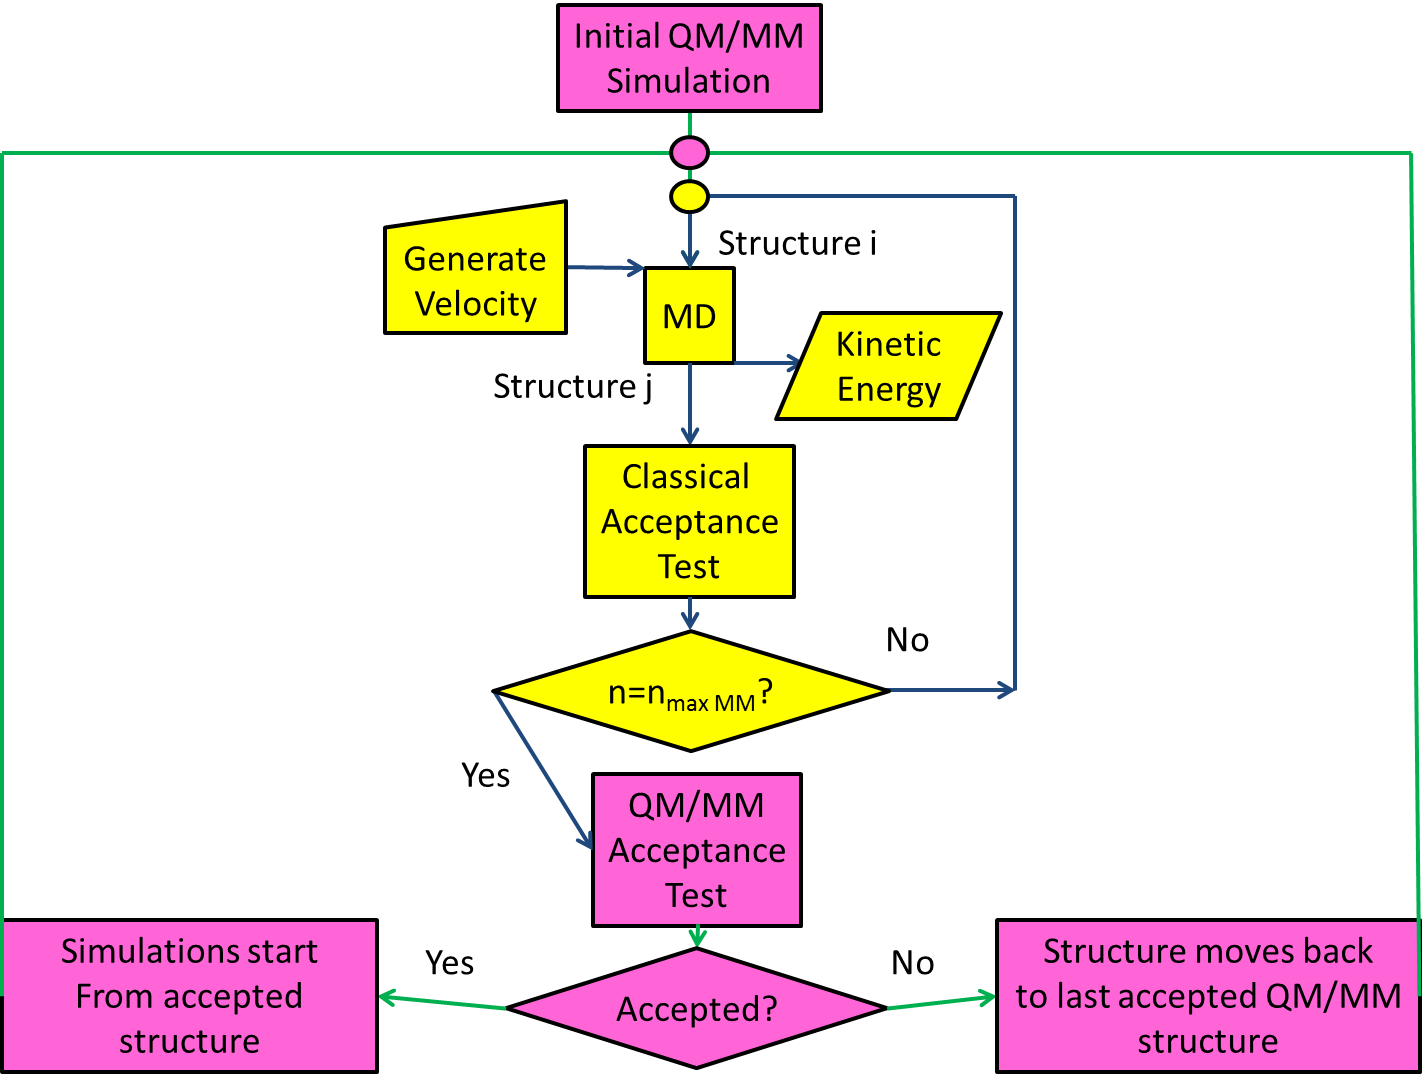
\includegraphics[width=18cm]{flow_chart.png}
\captionof{figure}{A flow chart describing how the method accepts to the QM/MM level, the inner loop (yellow and blue) represents hybrid Monte Carlo, the outer loop (pink and green) is the QM/MM level}\label{fig:flowchart}
\end{center}

\subsection{Stratification}

In order to make the transition from MM to QM/MM smoothly additional $\lambda$ steps can be introduced.  To do this, a simulation is performed in an identical fashion as previously described, with the only exception within the $\Delta \Delta U $ of equation \ref{eq:delta_delta_u}.  Where $U_{QM/MM}(\lambda)$ becomes $U_{QM/MM}(\lambda) = (1-\lambda) U_{classical} + (\lambda) U_{QM/MM}$.

The free energy is then obtained using thermodynamic integration (TI),

\begin{eqnarray}
\ \Delta G &=& \int_{0}^{1} d \lambda \left\langle \frac{\partial U (\lambda)}{\partial \lambda} \right\rangle_{\lambda} \nonumber \\
\frac{\partial U(\lambda)}{\partial \lambda} &=& U_{QM/MM}-U_{classical} \nonumber \\
\Delta G &=& \int_{0}^{1} d \lambda \left\langle U_{QM/MM}-U_{classical} \right\rangle_{\lambda} \nonumber
\end{eqnarray}

\subsection{Transitioning to the full QM}

By making the assumption that the $U_{QM/MM}$ ensemble is an accurate representation of the $U_{QM}$ ensemble, the transition from QM/MM to QM is simple.  To perform this perturbation, the energy differences $U_{QM}-U_{QM/MM}$ are calculated then the Zwanzig equation can be used as shown in equation \ref{eq:Zwanzig}.

\section{Methods}

\subsection{Classical details}

All parameters for non-waters, unless otherwise specified, were obtained using antechamber \cite{antechamber}.  The equilibration procedure was undertaken within Gromacs v4.6.2 \cite{ref_gromacs} using the leapfrog integrator and is as follows.  For ethane and ethanol in 448 and 450 waters respectively and alanine dipeptide in vacuum, structures were initially minimised with the steepest descent algorithm for 5000 steps with a cutoff of 11 \AA{}, electrostatics were treated with PME and a cut-off method was used for Van der Waals interactions.  Following this, a 500 ps simulation in the canonical ensemble was run using a timestep of 1 fs, the Berendsen thermostat was used to heat the system smoothly to 300 K, finally a 1 ns isothermal-isobaric simulation was performed using the Berendsen barostat.  After equilibration the box size decreased such that only a maximum of 8 \AA{} cut-off had to be used for the non-bonded interactions.

The water model used was initially a flexible SPC model described by Wu et al. \cite{flexible_spc}.  This was used as it should represent a quantum ensemble more accurately.

\begin{center}
\begin{table*}[ht]
{
\hfill{}
\begin{tabular}{c | c | c }
\hline 
Parameter & TIP3P & Flexible SPC \\ 
\hline 
r$_{OH}$ nm & 0.09572 & 0.10120 \\
\hline 
$\theta$ deg & 104.52 & 113.24 \\
\hline 
k$_a$ kcal/mol-rad$^2$ & 836.8 & 317.6 \\
\hline 
k$_b$ kcal/mol-nm & 462750.4 & 443153.4 \\
\hline 
$\epsilon$ kJ/mol & 0.635968 & 0.650299 \\
\hline 
$\sigma_{\infty}$ \AA & 0.315075 & 0.316549 \\
\hline 
q$_{O}$ e & -0.834 & -0.20 \\
\hline 
q$_{H}$ e & 0.417 & 0.410 \\
\hline 
\end{tabular}}
\hfill{}
\caption{Comparison of parameters for TIP3P water and flexible SPC}
\label{table:TIP3P_vs_SPC}
\end{table*}
\end{center}

The process for N$_2$ in vacuum was similar, although the pressure equilibration was skipped and a cutoff method was used for long range electrostatics.  N$_2$ in varying solvents (Ar, CH$_4$ and TIP3P water) was equilibrated following the above procedure, although a cutoff method was used for long range electrostatics within Ar and the parameters for Ar were taken from reference \cite{argon_params}.

The equilibration for cyclodextrin for the minimisation and isothermal-isobarric equilibration followed the above process, the simulation within the canonical ensemble differed slightly, in that the system was heated over 500ps and then allowed to run at 300K for an additional 1.5 ns.

The classical simulations within hybrid Monte Carlo were performed using the velocity-verlet algorithm, with a 0.25 fs timestep, the reason for such a small timestep can be seen in figure \ref{fig:timestep}.  Which shows the effect of changing the timestep for an MD simulation run 3 times.  The overall energy is conserved, but the fluctuations cause a lower classical acceptance rate when any larger timestep is used.  Each simulation is run for 20 ps and for the ethane and ethanol in water systems, 200 steps of pure hybrid Monte Carlo was performed as equilibration, following this, only a single classical simulation is run between QM/MM simulations.  The method was later simplified and details of this can be found in a forthcoming section.  When this simplification took place, it was found sufficient to only use 100 steps accepting to a classical N.V.T. ensemble as equilibration.

\begin{center}
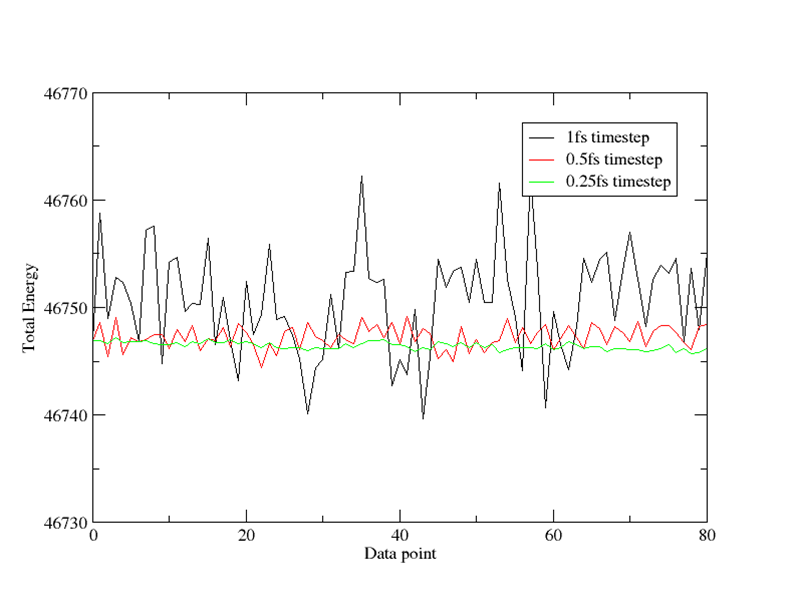
\includegraphics[width=15cm]{timestep_choice.png}
\captionof{figure}{Running an MD simulation using different timesteps to show fluctuations of the total energy in the microcanonical ensemble}\label{fig:timestep}
\end{center}


\subsection{QM details}

The quantum energies were calculated with two pieces of software, for testing NWCHEM \cite{nwchem} was used, then in order to move to fully quantum description ONETEP \cite{ONETEP} was used.  In both cases 100 steps of equilibration was initially performed, this involved 100 applications of the acceptance test.

When using NWCHEM, the exchange-correlation functionals of pbe96 were used with a cc-pvtz basis set for all atoms.  The setup for ONETEP, in the case of N$_2$, was that 4 NGWFs were used each being 7 bohr.  For ethane, ethanol, alanine dipeptide and cyclodextrin 4 NGWFs were used on heavy atoms and 1 for light atoms, all were 8 bohr and in both cases a kinetic energy cutoff of 800eV was used.

\section{Results}

\subsection{A Comparison of Methods While modifying the Force Field} \label{sec:N2_modification1}

A simple test system of N$_2$ in vacuum was selected to show the accuracy of the generated QM ensemble, when applying the Metropolis-Hastings criterion in comparison to the direct method of extracting snapshots from an MD trajectory at regular intervals and applying a single step free energy perturbation to the QM level.  The advantage of such a simple test system is that there is no need to define a classical region, meaning that we accept into a purely quantum ensemble.

For simplicity, the snapshots required for the single step perturbation approach (SSP) were taken from the ensemble when $\lambda$=0 of the Metropolis-Hastings applied method (MHA).  These snapshots accurately represent the classical canonical ensemble.

All parameters were obtained for N$_2$ from antechamber \cite{antechamber} with the exception of the equilibrium bond length which was set to the experimental length of 1.098 \cite{nist}.  The bond length within the force field was then increased in increments of 0.01 \AA{} and the effect on the proposed quantum ensemble was observed.  The results can be seen in table \ref{table:N2_force_field}.

\begin{center}
\begin{table*}[ht]
{
\hfill{}
\begin{tabular}{c | c | c | c}
\hline 
1.098 & SSP & \multicolumn{2}{c}{MHA} \\ 
\hline 
+ & Average Bond Length & Average Bond Length & Acceptance at $\lambda$=1 \\ 
\hline 
0.00 & 1.104 & 1.104 & 61.2 \\ 
\hline
0.01 & 1.110 & 1.104 & 64 \\ 
\hline 
0.02 & 1.120 & 1.105 & 50.4 \\ 
\hline 
0.03 & 1.130 & 1.103 & 35.6 \\ 
\hline 
0.04 & 1.138 & 1.110 & 28.4 \\ 
\hline 
0.05 & 1.149 & 1.113 & 16.6 \\ 
\hline 
0.06 & 1.159 & 1.100 & 7.0 \\ 
\hline 
0.07 & 1.169 & 1.100 & 2.2 \\ 
\hline 
0.08 & 1.179 & N/A & 0.0 \\ 
\hline 
0.09 & 1.188 & 1.117 & 1.0 \\ 
\hline 
0.10 & 1.197 & N/A & 0.0 \\ 
\hline 
\end{tabular}}
\hfill{}
\caption{The effect on the average bond length (shown in \AA) of the quantum ensemble when applying SSP and MHA and the acceptance rate (\%) of MHA at $\lambda$=1}
\label{table:N2_force_field}
\end{table*}
\end{center}

As expected, taking snapshots directly from an MD trajectory when the force field is parameterised badly, produces a poor representation of a quantum ensemble, which can be seen by examining the average bond lengths of table \ref{table:N2_force_field}.  However, when structures have to go through an acceptance criterion, as in MHA, the average bond length is conserved close to the experimental value.  By forcing the classical and quantum configurational space to overlap less, the acceptance at $\lambda$=1 is drastically effected, in some cases no structures were accepted post-equilibration.   This shows the acceptance rate is a good way to gauge how well the force field represents the quantum region: if the acceptance rate is very low then the force field is badly paramterised.  In a simple system such as this, identifying which parameter is the main cause of the poor acceptance rate is trivial, however, when moving to larger systems this will be highly non-trivial.  So, although the issue is identified the solution remains difficult to obtain.

The free energies of moving from the MM potential to the QM potential were then calculated and are shown in figure \ref{fig:extended_thermodynamic_cycle}.


%Change method 1 and method 2 to SSP and MHA, also consider making figures with PMF attached to free energies
%\begin{figure*}
\begin{center}
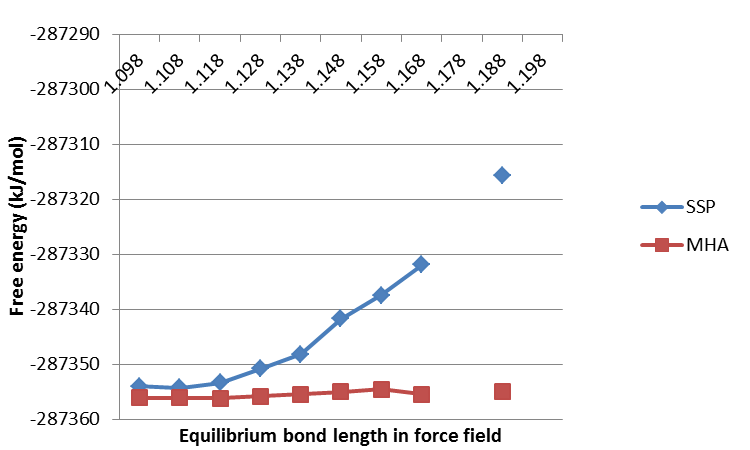
\includegraphics[width=15cm]{N2_free_energy_compare.png}
\captionof{figure}{Free energy as a function of the bond length when moving from MM to QM for N$_2$ in vacuum}\label{fig:N2_Free_energy}
\end{center}
%\end{figure*}

It is apparent by examination of figure \ref{fig:extended_thermodynamic_cycle} that the free energies diverge from each other as the equilibrium bond length is increased in the classical potential.  The explanation for this is found when considering the potential of mean force (PMF) plots produced when using $\lambda$ windows.  These are shown in figure \ref{fig:N2_PMF}.

%\begin{figure*}
\begin{center}
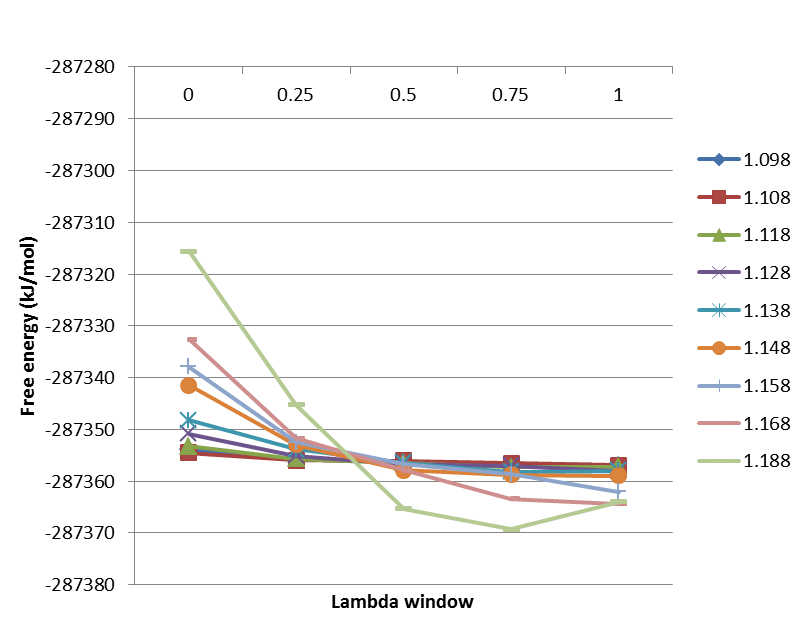
\includegraphics[width=15cm]{N2_free_energy_pmf.png}
\captionof{figure}{PMFs for the free energy as a function of the bond length when moving from MM to QM for N$_2$ in vacuum when applying MHA}\label{fig:N2_PMF}
\end{center}
%\end{figure*}

The Zwanzig equation (equation \ref{eq:Zwanzig}) assumes the PMF will be a straight line between the MM ($\lambda=0$) and QM ($\lambda=1$).  This assumption proves to be catastrophic to the free energies as the force field parameters move from the ideal values.  These results provide us with confidence that the MHA method can improve upon the results obtained when using the SSP method.  The next section applies these methods to more realistic test systems.

\subsection{Generating a QM/MM ensemble}

After the promising results when using N$_2$, more realistic test systems were chosen to be ethane in 448 waters and ethanol in 450 waters.  The introduction of water now provides us with the classical region within the ONIOM \cite{oniom} approach, so only the ligand is treated quantum mechanically.  For testing purposes, initially NWCHEM was used to calculate the quantum ligand.  This was later changed to ONETEP so the transition to full QM could be performed.  The NWCHEM results will be shown first followed by results obtained when using ONETEP, then the following section will cover the perturbation to the full QM.

To evaluate how converged the free energy between the classical and QM/MM ensembles are, A and B within figure \ref{fig:extended_thermodynamic_cycle} are both set to be the same, i.e. when using ethane in 448 waters both A and B are ethane in 448 waters.  The alchemical mutation usually required to obtain the free energy between these systems is then equal to 0.  Two simulations are then performed from MM to QM/MM (run 1 and run 2) and the free energy compared.  First the results for ethane in 448 waters are shown.

\begin{center}
\begin{table*}[ht]
{
\hfill{}
\begin{tabular}{c | c | c | c}
\hline 
 & SSP & \multicolumn{2}{c}{MHA} \\ 
\hline 
 & Free Energy & Free Energy & Acceptance at $\lambda$=1 \\ 
\hline 
Run 1 & -209340.77 & -209342.23 & 41.80 \\ 
\hline
Run 2 & -209340.83 & -209342.42 & 44.80 \\ 
\hline 
Difference & -0.06 & 0.18 &  \\ 
\hline 
\end{tabular}}
\hfill{}
\caption{Free energy convergence moving from MM to QM/MM for ethane in 448 waters, free energies shown in kJ/mol and acceptance is shown as \%}
\label{table:ethane_free_energy_nwchem}
\end{table*}
\end{center}


In this case, both methods prove to converge the free energy to within thermal error ($k_BT$).  Figure \ref{fig:ethane_PMF_nwchem} shows why both methods converge well.  The PMFs are both almost straight lines, the fluctuation in the PMF of run 1 shows is representative of the stochastic nature of the MHA method.

\begin{center}
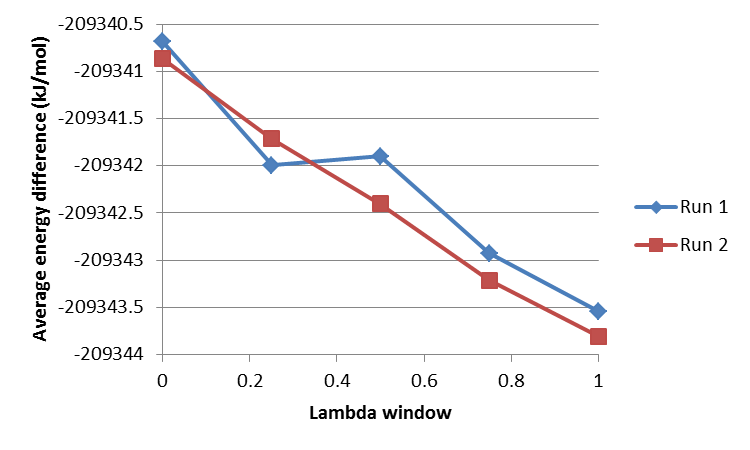
\includegraphics[width=15cm]{ethane_free_energy_nwchem.png}
\captionof{figure}{PMFs for the free energy for the two MHA runs for ethane in 448 waters using NWCHEM for the quantum region}\label{fig:ethane_PMF_nwchem}
\end{center}

To ensure convergence of the free energy shown for run 1, additional $\lambda$ values were introduced at 0.18, 0.35, 0.6 and 0.88.  The PMF was then plotted and is shown in figure \ref{fig:ethane_PMF_nwchem_more_lambda}

\begin{center}
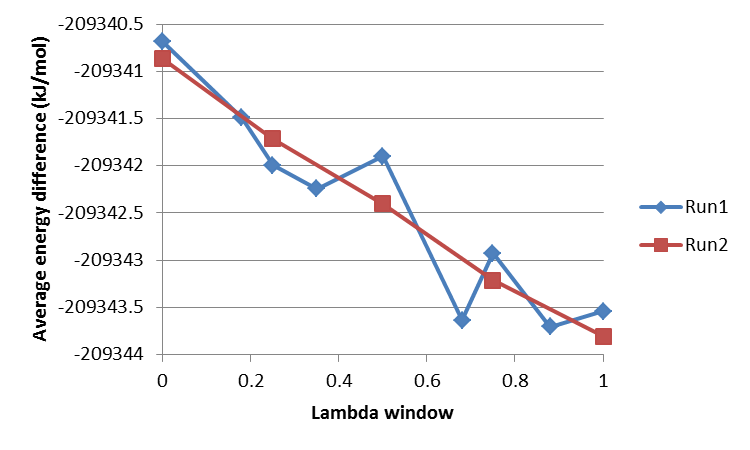
\includegraphics[width=15cm]{ethane_free_energy_nwchem_more_lambda.png}
\captionof{figure}{PMFs for the free energy for the two MHA runs for ethane in 448 waters using NWCHEM for the quantum region, with additional $\lambda$ windows for run 1}\label{fig:ethane_PMF_nwchem_more_lambda}
\end{center}

The fluctuations within figure \ref{fig:ethane_PMF_nwchem_more_lambda} run 1, again show the stochastic nature of the method.  However, by introducing these additional $\lambda$ steps the free energy for run 1 changes from -209342.23 kJ/mol to -209342.43 kJ/mol, which means the difference between run 1 and run 2 free energies is now 0.01 kJ/mol, proving convergence.

The method was then applied to ethanol in 450 waters and the results can be seen in table \ref{table:ethanol_free_energy_nwchem}.

\begin{center}
\begin{table*}[ht]
{
\hfill{}
\begin{tabular}{c | c | c | c}
\hline 
 & SSP & \multicolumn{2}{c}{MHA} \\ 
\hline 
 & Free Energy & Free Energy & Acceptance at $\lambda$=1 \\ 
\hline 
Run 1 & -406688.60 & -406693.31 & 16.80 \\ 
\hline
Run 2 & -406688.65 & -406693.00 & 18.60 \\ 
\hline 
Difference & 0.05 & -0.31 &  \\ 
\hline 
\end{tabular}}
\hfill{}
\caption{Free energy convergence moving from MM to QM/MM for ethanol in 450 waters, free energies shown in kJ/mol and acceptance is shown as \%}
\label{table:ethanol_free_energy_nwchem}
\end{table*}
\end{center}

Both methods converge the free energy for ethanol in 450 waters, although interestingly the acceptance rates are considerably lower than those for ethane in 450 waters.  The change in acceptance rate is attributed to the presence of the alcohol group within ethanol, perhaps the OH bond vibration is modelled poorly by the classical region.  

\begin{center}
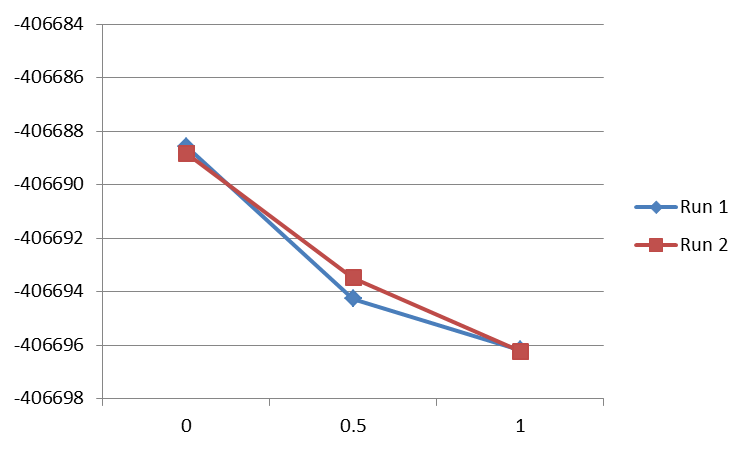
\includegraphics[width=15cm]{ethanol_free_energy_nwchem.png}
\captionof{figure}{PMFs for the free energy for three MHA runs for ethanol in 450 waters using NWCHEM for the quantum region}\label{fig:ethanol_PMF_nwchem}
\end{center}

The PMFs moving between MM and QM/MM can be see in figure \ref{fig:ethanol_PMF_nwchem}, which confirms how well converged the free energies are.

These results have shown that it is possible to go to a QM/MM level and converge the free energy, the next step is to perturb to the full QM ensemble.  Because of this, the process of generating QM/MM ensembles was repeated using ONETEP.  Only 3 $\lambda$ windows were used with ONETEP, $\lambda=0, 0.5, 1$.  Figure \ref{fig:ethane_PMF_ontep} shows the obtained PMFs.

\begin{center}
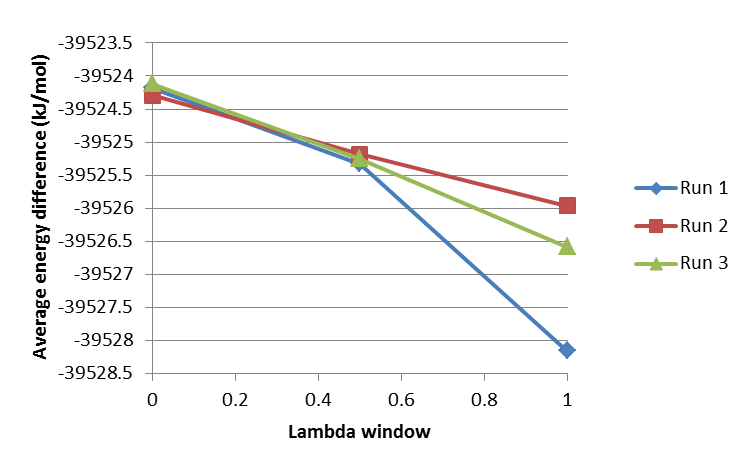
\includegraphics[width=15cm]{ethane_free_energy_onetep.png}
\captionof{figure}{PMFs for the free energy for three MHA runs for ethane in 448 waters using ONETEP for the quantum region}\label{fig:ethane_PMF_ontep}
\end{center}

Examination of figure \ref{fig:ethane_PMF_ontep} shows a difference of 2 kJ/mol within the average energy difference of $\lambda=1$.  This is still within thermal error, but can be explained by, again, considering the stochastic nature of the method.  Even taking these differences to account the convergence of the free energies is largely unaffected (table \ref{table:ethane_free_energy_onetep}) with the largest difference being just under 1 kJ/mol.  

\begin{center}
\begin{table*}[ht]
{
\hfill{}
\begin{tabular}{c | c | c | c}
\hline 
 & SSP & \multicolumn{2}{c}{MHA} \\ 
\hline 
 & Free Energy & Free Energy & Acceptance at $\lambda$=1 \\ 
\hline 
Run 1 & -39524.18 & -39525.18 & 34.09 \\ 
\hline
Run 2 & -39524.28 & -39525.15 & 51.80 \\ 
\hline 
Run 3 & -39524.19 & -39524.19 & 43.00 \\ 
\hline 
Difference & 0.10 & 0.99 &  \\ 
\hline 
\end{tabular}}
\hfill{}
\caption{Free energy convergence moving from MM to QM/MM, free energies shown in kJ/mol and acceptance is shown as \% and the difference is the largest difference between the values}
\label{table:ethane_free_energy_onetep}
\end{table*}
\end{center}

The method was then again applied to ethanol in solvent, the results can be see in table \ref{table:ethanol_free_energy_onetep}.  A simulation was then performed at $\lambda=1$ restraints were applied to any bond that involved hydrogen.  The resulting acceptance rate was 28.36\%, which is an increase of approximately 6\% than when these bonds are allowed to vibrate.  Although a higher acceptance, using flexible hydrogen bonds will be able to sample more structures, so these simulations will be used for analysis.

\begin{center}
\begin{table*}[ht]
{
\hfill{}
\begin{tabular}{c | c | c | c}
\hline 
 & SSP & \multicolumn{2}{c}{MHA} \\ 
\hline 
 & Free Energy & Free Energy & Acceptance at $\lambda$=1 \\ 
\hline 
Run 1 & -81550.56 & -81555.02 & 22.40 \\ 
\hline
Run 2 & -81551.09 & -81555.44 & 21.0 \\ 
\hline 
Difference & 0.53 & 0.42 &  \\ 
\hline 
\end{tabular}}
\hfill{}
\caption{Free energy convergence moving from MM to QM/MM for ethanol in 450 waters, free energies shown in kJ/mol and acceptance is shown as \%}
\label{table:ethanol_free_energy_onetep}
\end{table*}
\end{center}

Free energies shown in table \ref{table:ethanol_free_energy_onetep} are again converged with a lower acceptance rate than the acceptance rate for ethane.  The PMFs can be seen in figure \ref{fig:ethanol_PMF_onetep}.

\begin{center}
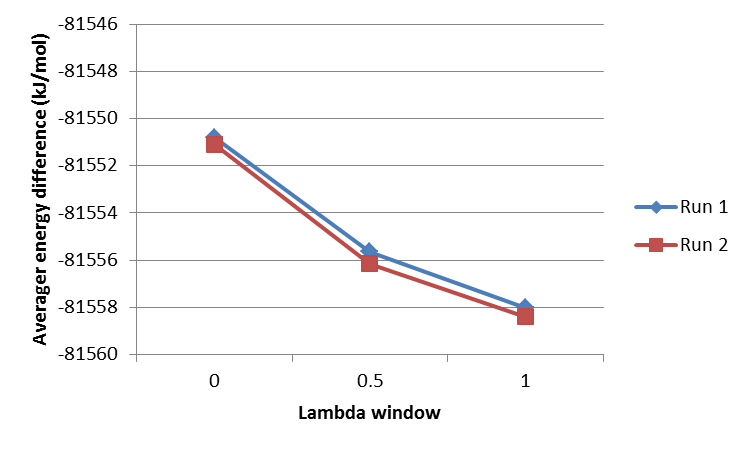
\includegraphics[width=15cm]{ethanol_free_energy_onetep.png}
\captionof{figure}{PMFs for the free energy for three MHA runs for ethanol in 450 waters using ONETEP for the quantum region}\label{fig:ethanol_PMF_onetep}
\end{center}

As expected, these results show convergence comparable to that obtained when using NWCHEM.

\subsection{Perturbation to full QM}


\begin{center}
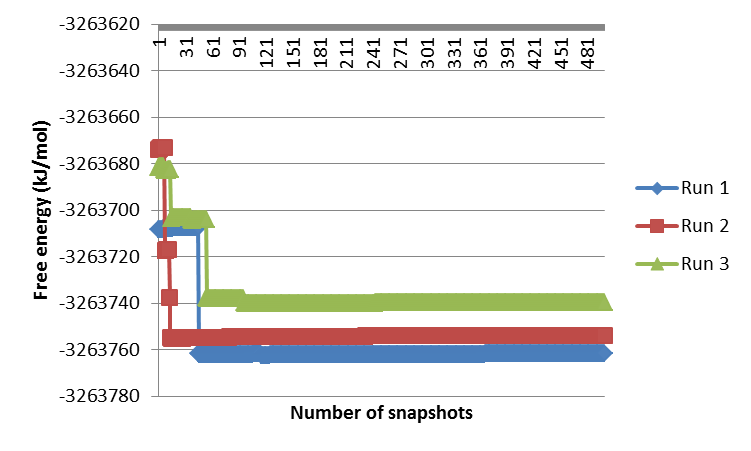
\includegraphics[width=15cm]{ethane_free_energy_onetep_fullqm.png}
\captionof{figure}{Free energy as a function of the number of snapshots when moving from the QM/MM to the QM for ethane in 448 waters}\label{fig:ethane_fullqm_onetep}
\end{center}

\begin{center}
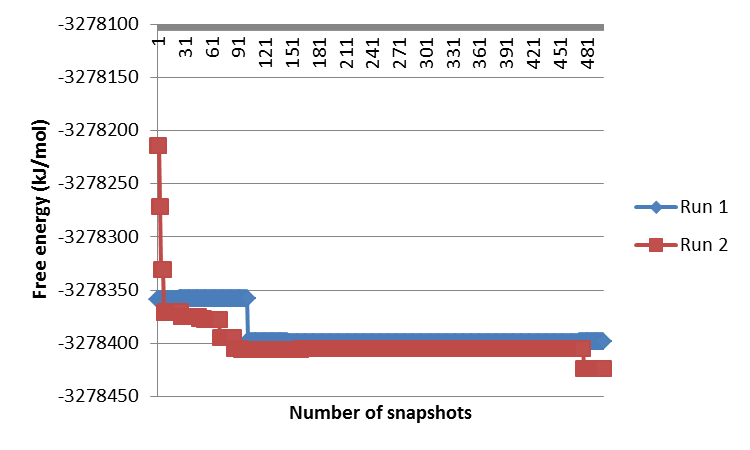
\includegraphics[width=15cm]{ethanol_free_energy_onetep_fullqm.png}
\captionof{figure}{Free energy as a function of the number of snapshots when moving from the QM/MM to the QM for ethanol in 450 waters}\label{fig:ethanol_fullqm_onetep}
\end{center}


Once the QM/MM ensemble of structures was generated, the next step was to perturb to the full QM, shown in figure \ref{fig:ethane_fullqm_onetep} and figure \ref{fig:ethanol_fullqm_onetep}.  The ``sawtooth'' shape of the graph shows an issue with sampling \cite{good_practice_free_energy}.  This shows that the QM/MM ensemble is not representative of the QM ensemble.  In order to better represent a quantum ensemble, either the classical potential needs to be modified or the QM/MM description needs to be improved.

\subsection{Extending the Quantum Region}

In order to remove the sampling issues causing the ``sawtooth'' shape within figure \ref{fig:ethane_fullqm_onetep} and \ref{fig:ethanol_fullqm_onetep} the quantum region within the QM/MM was extended to some include water molecules.  To decide how many water molecules to include the radial distribution function (RDF) was calculated for a 20ps simulation of ethane in 448 water and can be seen in figure \ref{fig:RDF}.

\begin{center}
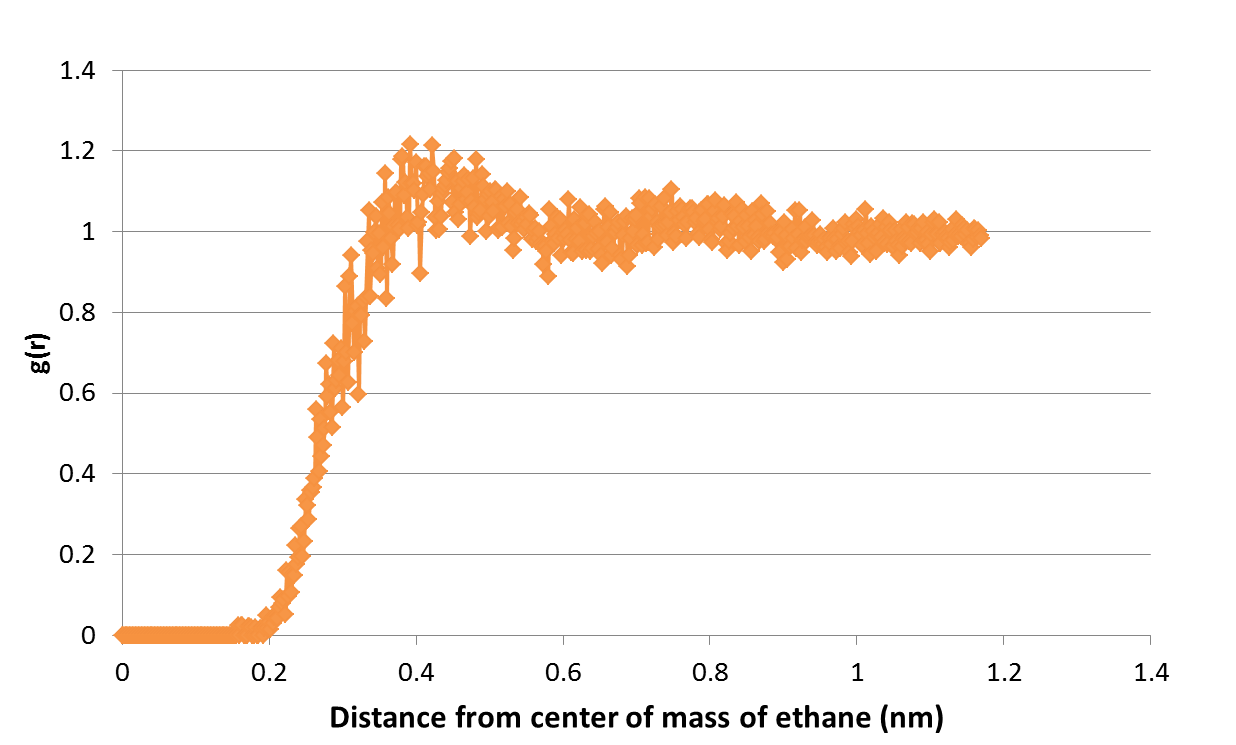
\includegraphics[width=15cm]{radial_distribution_function.png}
\captionof{figure}{Radial Distribution Function for a 20 ps simulation of ethane in 448 water}\label{fig:RDF}
\end{center}

As a first attempt to represent the QM configurational space better, the first solvation sphere was selected to be included within the quantum region.  By examination of figure \ref{fig:RDF} it can be seen that the first solvation sphere ends approximately at 6 \AA{}.  The same simulation used to calculate the RDF was then used to calculate how many waters were within 6\AA{} of ethane (using centre of mass).  The result shows a maximum of 54 waters.  The quantum region was then selected to be ethane and the closest 54 waters within the mechanically embedded remaining 394 waters.

The simulations (two runs) were originally set up to obtain 600 quantum structures using ONETEP, as before, but after 380 both were cancelled.  The reason for this is that after the 100 equilibration steps not a single structure was accepted, which is due to fluctuations of hundreds of kJ/mol within the calculated quantum energies.

The reason a set number of water was chosen, rather than a fixed cutoff was to avoid fluctuations due to different numbers of water within the quantum region, but, regardless of this, fluctuations are present.  The previous  results show that the quantum energy fluctuation for ethane is within acceptable range (judging by the 40\% acceptance rate).  This leads to the conclusion that the fluctuations are either caused by the interaction between the water and ethane or the intramolecular energy of the water or the intermolecular interaction between the water molecules.  As such each water within a snapshot was extracted and for speed the quantum energy was calculated using NWCHEM.  The resulting energies had a range of 70.14 kJ/mol showing a massive range of intramolecular energies.  This fluctuation in energy means that the flexible water model used isn't suitable to sample quantum conformational space.

The results for ethanol in water showed an improvement of around 6\% when using SHAKE.  This large range in intramolecular energy of water is too high to obtain a reasonable acceptance.  Fully flexible models were used in order to not limit the favourable quantum regions that would otherwise not be sampled using SHAKE.  However, SHAKE must be used in order to accept any structures.


\subsection{A simplification of the method}

As stated in the theory section, hybrid Monte Carlo allows the generation of an ensemble in a desired potential, that differs from the potential used to sample configurations.  By considering this, it is possible to avoid accepting to a classical canonical ensemble, then moving to the QM/MM ensemble using two different acceptance tests; and building an ensemble on an ensemble.  Instead, it is possible to change the acceptance criterion (equation \ref{eq:hamiltonian_acceptance}) to include the QM/MM potential energy and $\lambda$ windows could be introduced in the same manner as previously shown.  This new implementation avoids the need for a nested loop and is conceptually simpler.  This method can be considered by examining the inner loop (yellow and blue) of figure \ref{fig:flowchart}, where instead of the classical acceptance test you use the modified acceptance test, which makes the move to the QM/MM level redundant (in the outer loop).

To validate the application of hybrid Monte Carlo (HMC) in this way, the test involving modifying the equilibrium bond length of N$_2$, performed in section \ref{sec:N2_modification1} was repeated, this time using ONETEP for the QM calculations.

\subsection{Applying HMC to N$_2$ while modifying the equilibrium bond length}

To validate this simplification of the method, the simple test of N$_2$ in vacuum while changing the equilibrium bond length used within the force field was performed again.  The results are shown in \ref{table:N2_force_field_simplification}.

\begin{center}
\begin{table*}[ht]
{
\hfill{}
\begin{tabular}{c | c | c | c}
\hline 
1.098 & SSP & \multicolumn{2}{c}{MHA} \\ 
\hline 
+ & Average Bond Length & Average Bond Length & Acceptance at $\lambda$=1 \\ 
\hline 
0.00 & 1.098 & 1.104 & 62.8 \\ 
\hline
0.01 & 1.109 & 1.106 & 62.0 \\ 
\hline 
0.02 & 1.121 & 1.107 & 54.2 \\   
\hline 
0.03 & 1.132 & 1.108 & 42.6 \\ 
\hline 
0.04 & 1.140 & 1.109 & 33.2 \\ 
\hline
\end{tabular}}
\hfill{}
\caption{The effect on the average bond length (shown in \AA) of the quantum ensemble when changing the equilibrium bond length within the force field. The acceptance rate is shown as a percentage and is for $\lambda$=1}
\label{table:N2_force_field_simplification}
\end{table*}
\end{center}

The results shown in table \ref{table:N2_force_field_simplification} show that this simplification of the method yields similar results to the more complex multi-stepping Monte Carlo used previously.  As before the free energy moving from MM to QM is shown for the two methods, SSP and MHA.

\begin{center}
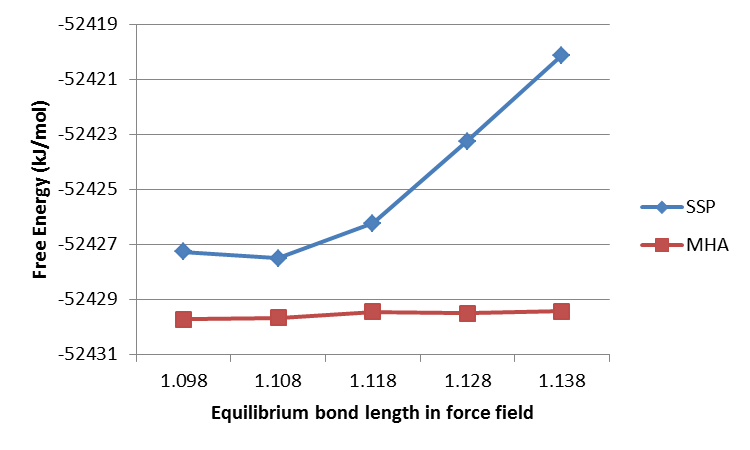
\includegraphics{N2_free_energy_compare2.png}
\captionof{figure}{Comparison of free energy calculated when using the SSP and MHA methods while changing the classical equilibrium bond length of N$_2$}\label{fig:N2_free_energy_compare}
\end{center}

\begin{center}
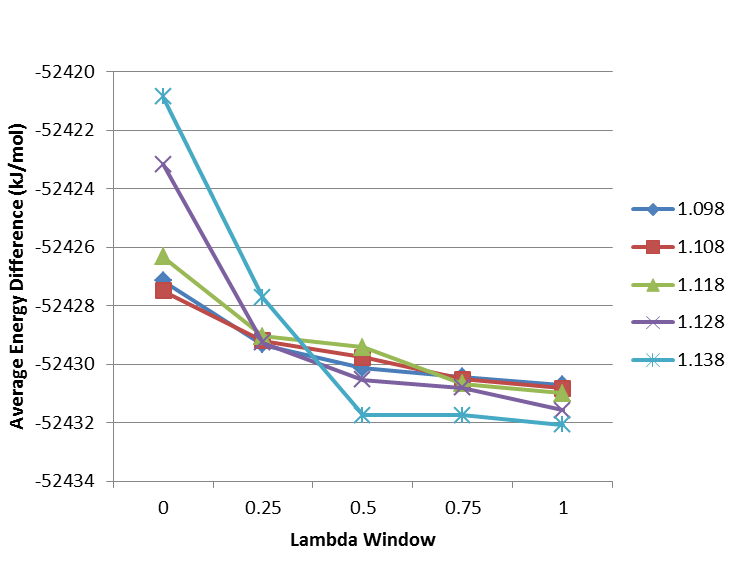
\includegraphics{N2_free_energy_pmf2.png}
\captionof{figure}{PMFs when moving from MM ($\lambda=0$) to QM ($\lambda=1$) for N$_2$ when altering the classical equilibrium bond length}\label{fig:N2_free_energy_pmf}
\end{center}

Both figure \ref{fig:N2_free_energy_compare} and \ref{fig:N2_free_energy_pmf} show similar trends to the previous method, but with different energy values.  The difference in the energy is solely due to using ONETEP within this simplification of the method, whereas previously NWCHEM was used.  These results show that the simplified version of MHA is just as accurate as the previous method.

Previously we showed convergence issues when perturbing from QM/MM to QM.  In order to identify the cause of these convergence issues, N$_2$ in solvents of increasing complexity was used.  These solvents were Ar, CH$_4$ and TIP3P water.

\subsection{N$_2$ in Ar}

As mentioned above, the first test is the simplest as there is no electrostatic or polarisation terms required.  Because of this the classical potential should provide an accurate description of the ensemble.  The first step to calculate the free energies is to generate ensembles at different $\lambda$ values between the MM and QM/MM descriptions for the system.  The resultant PMFs in figure \ref{fig:N2_free_energy_pmf_Ar} shows excellent convergence between the two simulation runs, the difference between the free energies for these runs was 0.09 kJ/mol.

\begin{center}
\includegraphics{N2_AR_MM_to_QM-MM.png}
\captionof{figure}{PMFs when moving from MM ($\lambda=0$) to QM/MM ($\lambda=1$) for N$_2$ in 250 Ar}\label{fig:N2_free_energy_pmf_Ar}
\end{center}

Using the structures that were accepted at $\lambda=1$ (the QM/MM ensemble), the fully QM energy was calculated on the entire system.  Then a single step perturbation was performed, the produced free energy was then added to the free energy required to move from an MM description to a QM/MM description of the system.  The resultant values can be seen in table \ref{table:N2_AR_MM_to_QM}.

\begin{center}
\begin{table*}[ht]
{
\hfill{}
\begin{tabular}{ c | c }
\hline 
  & Free Energy (kJ/mol)   \\  
\hline 
Run 1 & -2297316.80  \\ 
\hline
Run 2 & -2297315.90  \\ 
\hline 
Difference & 1.10  \\ 
\hline 
\end{tabular}}
\hfill{}
\caption{Free energy when moving from MM to QM for N$_2$ in 250 Ar}
\label{table:N2_AR_MM_to_QM}
\end{table*}
\end{center}

This small difference within the free energies is within thermal error.  Further analysis of the free energy calculated between the QM/MM and QM was performed by increasing the number of snapshots included within the Zwanzig equation in increments of 1.  The produced graph will show if a single or a few snapshots are dominating the free energy.


\begin{center}
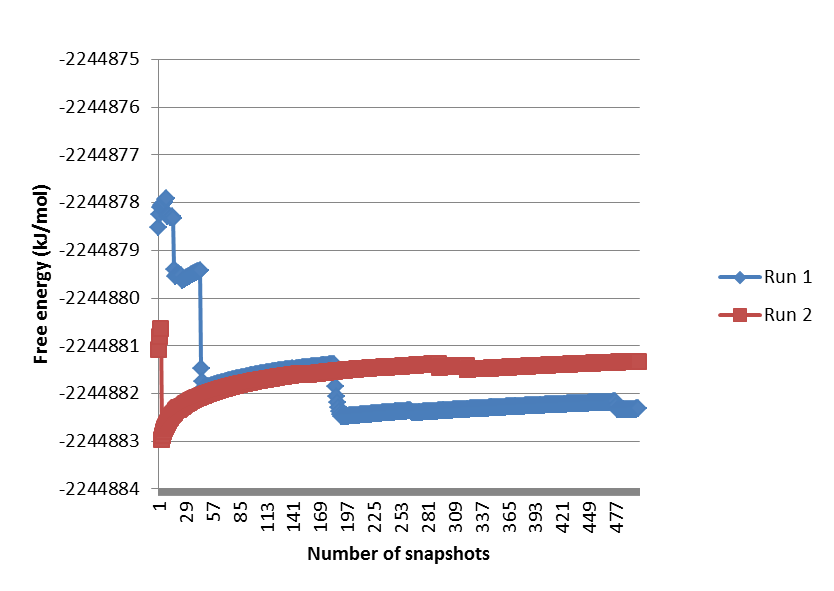
\includegraphics{N2_AR_QM-MM_to_QM.png}
\captionof{figure}{Increasing the number of snapshots included in the Zwanzig equation when perturbing from QM/MM to QM}\label{fig:N2_free_energy_zwanzig_Ar}
\end{center}

The results shown in figure \ref{fig:N2_free_energy_zwanzig_Ar} display a ``sawtooth'' shape which is characteristic of poor sampling \cite{good_practice_free_energy}.  However, the free energy for the two runs is similar because the changes within the free energy are small, which can be largely attributed to the simplicity of this system.  By increasing the complexity of the system, it is predicted that this ``sawtooth'' sampling will have a much larger effect on the free energy.


\subsection{N$_2$ in CH$_4$}

By introducing the solvent of 250 CH$_4$, there are now small partial charges and the complexity of the system is increased.  The intermolecular interactions are now no longer solely dispersion driven.  As before, first the free energy moving from an MM description to a QM/MM description was found.  

\begin{center}
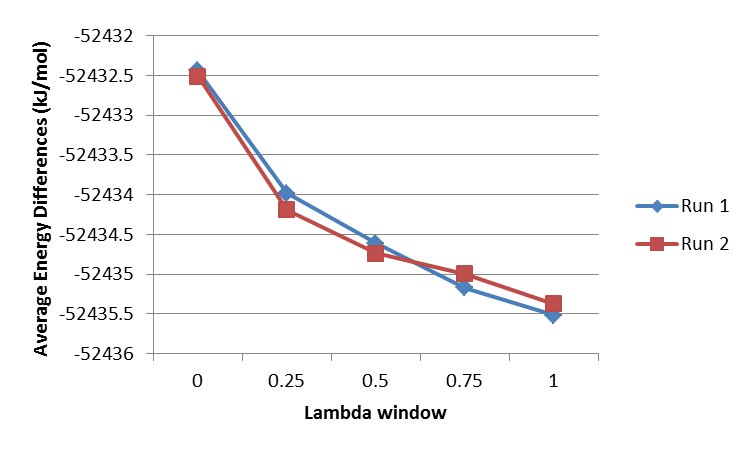
\includegraphics[width=15cm]{N2_CH4_MM_to_QM-MM.png}
\captionof{figure}{Free energy when moving from MM to QM for N$_2$ in 250 CH$_4$}\label{fig:N2_free_energy_pmf_CH4}
\end{center}

Figure \ref{fig:N2_free_energy_pmf_CH4} shows the two PMFs are almost identical and this is reflected in the 0.03 kJ/mol free energy difference between them.

\begin{center}
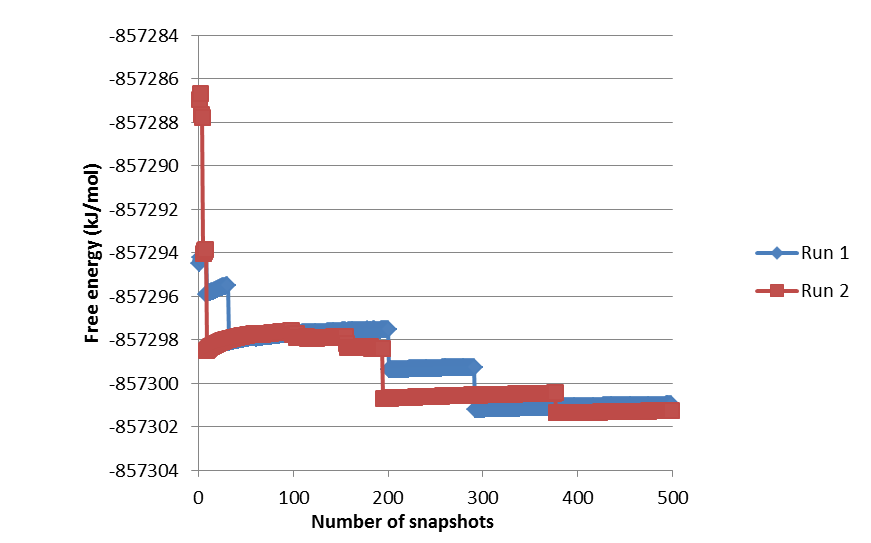
\includegraphics[width=15cm]{N2_CH4_QM-MM_to_QM.png}
\captionof{figure}{Increasing the number of snapshots included in the Zwanzig equation when perturbing from QM/MM to QM for N$_2$ in CH$_4$}\label{fig:N2_free_energy_zwanzig_CH4}
\end{center}

Performing the same analysis as before: increasing the number of snapshots included within the Zwanzig equation, figure \ref{fig:N2_free_energy_zwanzig_CH4} was produced.  The ``sawtooth'' shape is again present, but the final snapshots show no large changes in either simulation runs.  The final difference in the free energy when moving from MM to QM can be seen in table \ref{table:N2_CH4_MM_to_QM}.  This excellent agreement shows that the way the classical force field has modelled the intermolecular interactions here agrees well with the quantum description.


\begin{center}
\begin{table*}[ht]
{
\hfill{}
\begin{tabular}{ c | c }
\hline 
  & Free Energy (kJ/mol)   \\  
\hline 
Run 1 & -909735.43 \\ 
\hline
Run 2 & -909735.72 \\ 
\hline 
Difference & 0.29 \\ 
\hline 
\end{tabular}}
\hfill{}
\caption{Free energy when moving from MM to QM for N$_2$ in 250 CH$_4$}
\label{table:N2_CH4_MM_to_QM}
\end{table*}
\end{center}


\subsection{N$_2$ in TIP3P}

The final test system is the most complex and most interesting system.  By introducing a higher partial charge, electrostatics will be the main driving force for the intermolecular interactions and polarisation effects will be present.  Polarisation is included implicitly within the force field \cite{polarisable_force_field_russian}.  To keep the box size similar and using a realistic density, 499 waters were used.  The PMFs generated by moving from a classical to a QM/MM description are shown in figure \ref{fig:N2_free_energy_pmf_TIP3P}.  The convergence between the simulation runs was 0.12 kJ/mol.


\begin{center}
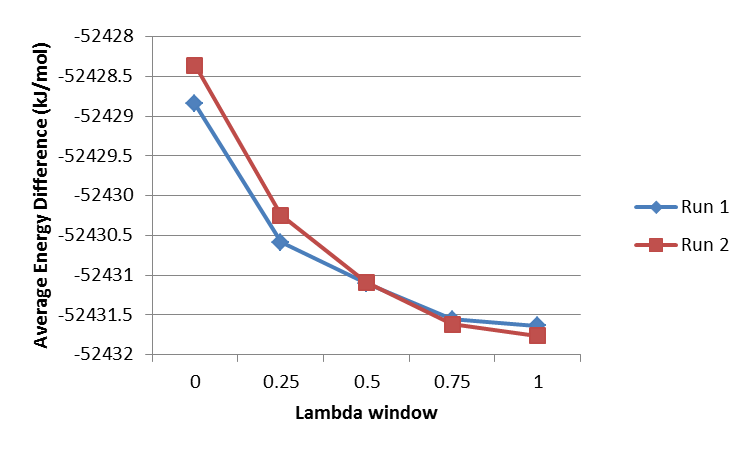
\includegraphics[width=15cm]{N2_TIP3P_MM_to_QM-MM.png}
\captionof{figure}{Free energy when moving from MM to QM/MM for N$_2$ in 499 water}\label{fig:N2_free_energy_pmf_TIP3P}
\end{center}

Next, the free energy between the QM/MM and full QM was calculated.  As before this was performed is a stepwise manner to ensure convergence, the results can be seen in figure \ref{fig:N2_TIP3P_QM-MM_to_QM}.  Again the ``sawtooth'' shape is present, and the two runs have not converged to a single value.  Also notice that the ``jumps'' in the graph are larger than in any other solvent, which implicates that the electrostatics have the largest effect on the convergence.  If this is the case then using a QM/MM description that uses electrostatic embedding instead of mechanical embedding should improve the quality of the ensemble at the QM/MM level.


\begin{center}
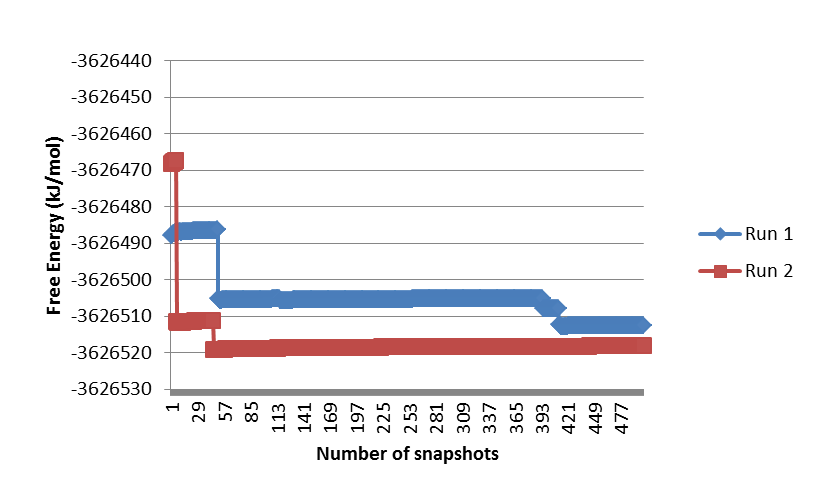
\includegraphics{N2_TIP3P_QM-MM_to_QM.png}
\captionof{figure}{Increasing the number of snapshots included in the Zwanzig equation when perturbing from QM/MM to QM for N$_2$ in TIP3P}\label{fig:N2_TIP3P_QM-MM_to_QM}
\end{center}

The total free energy moving from MM to QM can be seen in table \ref{table:N2_TIP3P_MM_to_QM}.

\begin{center}
\begin{table*}[ht]
{
\hfill{}
\begin{tabular}{ c | c }
\hline 
  & Free Energy (kJ/mol)   \\  
\hline 
Run 1 & -3678943.45 \\ 
\hline
Run 2 & -3678948.83 \\ 
\hline 
Difference & 5.38 \\ 
\hline 
\end{tabular}}
\hfill{}
\caption{Free energy when moving from MM to QM for N$_2$ in 250 CH$_4$}
\label{table:N2_TIP3P_MM_to_QM}
\end{table*}
\end{center}


Regardless of the solvent used convergence was achieved to the QM/MM level.  The perturbation the full QM displayed ``sawtooth'' shaped graphs, which are stereotypical of poor sampling.  This indicates that the QM/MM description is not close enough to the full QM description, which could be improved by using electrostatic embedding instead of the mechanical embedding used here.

The ``jumps'' within the graphs increase in size as the main intermolecular interactions between solute and solvent shift between dispersion and electrostatics, because of this electrostatic embedding was introduced to improve configurational overlap between the QM/MM and QM.

\subsection{Introducing electrostatic embedding}

For systems in vacuum or when mechanical embedding was used, equilibration was achieved rapidly.  However, the introduction of point charges led to slower equilibration.  In order to increase the speed at which this could be achieved, a classical equilibration was included initially, i.e. after the system had been minimised, heated and the box size equilibrated, a further classical equilibration was performed using HMC to accept to a classical NVT ensemble.

Although N$_2$ in various solvents has been used heavily as a test system, in order to appreciate the additional accuracy provided by using electrostatic embedding an solute that has a larger interaction with the solvent was chosen, in this case ethanol in 450 TIP3P water.  TIP3P was used because of the additional acceptance that occurred when comparing rigid with flexible waters previously.

However, it was found that once out of the 100 steps of classical equilibration and 100 steps of QM/MM equilibration, no snapshots were accepted.  By comparing the MM and QM potential energy figure \ref{fig:MM_to_QM_ethanol_450_tip3p_comparison} is produced.  Although the QM/MM Hamiltonian energy is used within the acceptance criterion, the potential energies of both QM/MM and MM can be compared because of the following relationship,

\begin{eqnarray}
\ \Delta H &=& (E_{QM}^j+E_{KIN}^j)-(E_{QM}^i+E_{KIN}^i) \\
\ &=& E_{QM}^j-E_{QM}^i + E_{KIN}^j - E_{KIN}^i \\
\ &=& E_{QM}^j-E_{QM}^i + E_{MM}^i - E_{MM}^j   \label{eq:kin_to_MM_relationship} \\
\ &=& (E_{QM}^j-E_{MM}^j) - (E_{QM}^i - E_{MM}^i) .
\end{eqnarray}

Where the step in equation \ref{eq:kin_to_MM_relationship} can be performed because the MD is performed in the microcanonical ensemble, i.e. (assuming no integrator errors) the difference in kinetic energy and classical potential energy will be equal and opposite, $\Delta E_{KIN}=-\Delta E_{MM}$.


\begin{center}
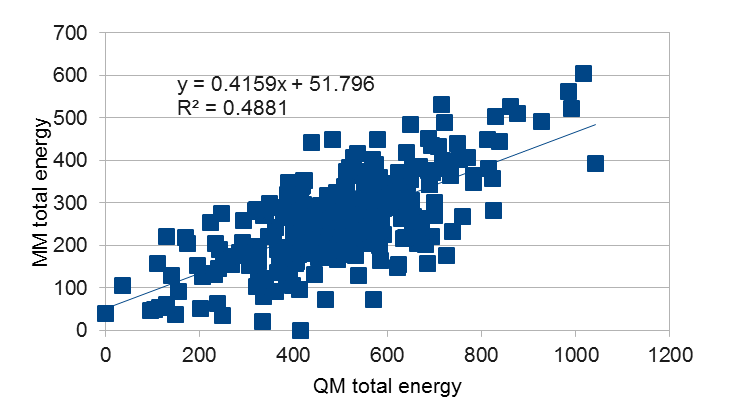
\includegraphics{MM_to_QM_ethanol_450_tip3p_comparison.png}
\captionof{figure}{Comparison of MM and QM/MM potential energy for ethanol in 450 TIP3P waters}\label{fig:MM_to_QM_ethanol_450_tip3p_comparison}
\end{center}

The positive correlation shown in figure \ref{fig:MM_to_QM_ethanol_450_tip3p_comparison} shows that there is a relationship between the potential energies, but the correlation is not high enough for a good acceptance rate.  However, this correlation can be drastically improved by including the classical dispersion within the QM/MM potential energy.  The result can be seen in figure \ref{fig:MM_to_QM+LJ_ethanol_450_tip3p_comparison}.


\begin{center}
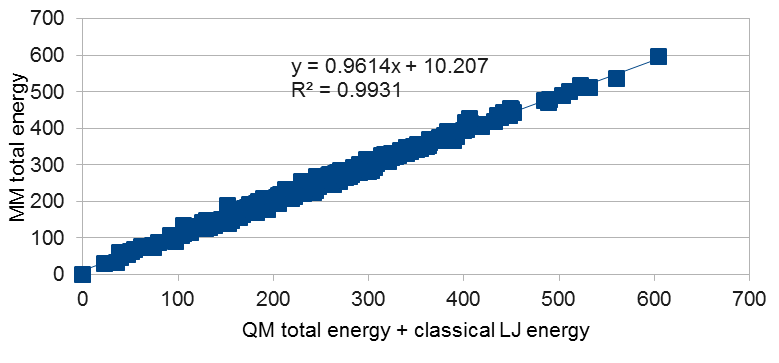
\includegraphics{MM_to_QM+LJ_ethanol_450_tip3p_comparison.png}
\captionof{figure}{Comparison of MM and QM/MM + LJ potential energy for ethanol in 450 TIP3P waters}\label{fig:MM_to_QM+LJ_ethanol_450_tip3p_comparison}
\end{center}

Even with an R$^2$ value of 0.99 the MM and QM/MM + LJ overlap is still insufficient to obtain any acceptance outside of the equilibration steps.  The reasoning for this becomes clear when examining figure \ref{fig:MM_and_QM_overlap} and \ref{fig:MM_and_QM_difference}.

\begin{center}
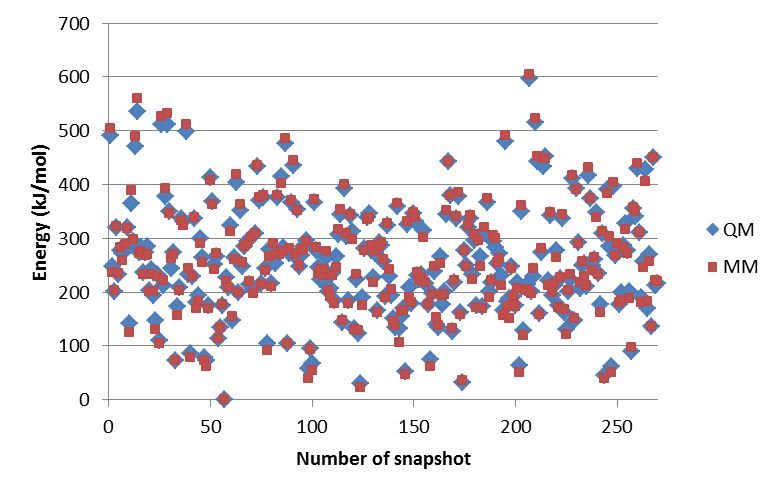
\includegraphics{MM_and_QM_overlap.png}
\captionof{figure}{Level of overlap between the MM and QM/MM+LJ, both have been shifted down so the lowest energy snapshots sit at 0}\label{fig:MM_and_QM_overlap}
\end{center}

\begin{center}
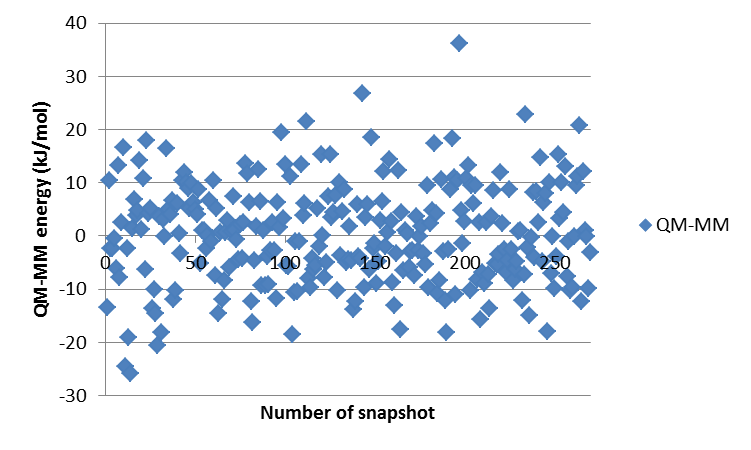
\includegraphics{MM_and_QM_difference.png}
\captionof{figure}{The difference between the QM/MM+LJ and MM potential energy, the average energy difference has been subtracted from each energy difference}\label{fig:MM_and_QM_difference}
\end{center}

These figures (figure \ref{fig:MM_and_QM_overlap} and \ref{fig:MM_and_QM_difference}) highlight a flaw in the method, if the QM/MM+LJ energy is lower than the MM energy in figure \ref{fig:MM_and_QM_overlap} then the energy difference is negative and is accepted, regardless of the true probability to select this snapshot from a QM/MM+LJ potential energy surface.  By examining the energy differences and subtracting the average energy difference, figure \ref{fig:MM_and_QM_difference} is produced, which shows a large number of the snapshots appearing around 0 kJ/mol.  This shows that the MM is, on the whole, a good representation of the QM/MM+LJ surface.  However, rare events cause a large negative energy difference, which then cause the simulation to get stuck.  For example, in figure \ref{fig:MM_and_QM_difference}, the lowest energy difference occurs very early on, as such after this snapshot no other is accepted.  This is caused by the inexact overlap between the MM and QM/MM+LJ.

There are several possible solutions to this issue, the first being to alter the force field to improve the level of overlap, alternatively the MC steps can be made much smaller to make use of the correlation between structures to ensure that energy differences are close together.


\subsubsection{Small MC Steps}

%Maybe MM to QM can come in here?

By lowering the movement of the system between subsequent snapshots the acceptance rate should increase.  In order to lower the movement, the length of the MD simulation used to generate structures was made shorter.  By lowering the time of the MD to 0.25fs, a single timestep, the acceptance for ethanol in 450 electrostatic embedded waters increases to 99\%.  The disadvantage with this is that each snapshot is correlated, so cannot give an accurate representation of the free energy.

Lowering the time between structures was tested on a larger system of cyclodextrin in complex with chlorobenzene in vacuum (figure \ref{fig:cyclodextrin_PhCl}).  Both MD lengths of 2 fs and 5 fs were tested, and in both cases the acceptance was below 10\%.

Although in theory using much smaller moves works, using a method like this will take a long time to converge the free energy, the bottleneck being the calculation of the QM/MM.

\begin{center}
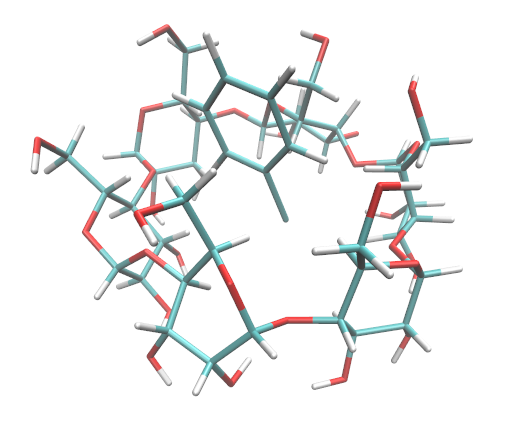
\includegraphics[width=10cm]{cyclodextrin_PhCl.png}
\captionof{figure}{Cyclodextrin bound to PhCl}\label{fig:cyclodextrin_PhCl}
\end{center}

\subsubsection{Altering the Force Field/Removing Degrees of Freedom}

In order to achieve higher acceptance rates, alterations to the force field were considered.  If the classical potential energy surface was a better match for the QM/MM potential energy surface, then the acceptance will increase.  In order to test this a simple system of ethanol in vacuum was used.

The quantum parameters were obtained by geometry optimisation.  The equilibrium values in the force field were then altered to match the values for the quantum optimised structure.  Table \ref{table:altering_force_field} shows the results of changing these values

\begin{center}
\begin{table*}[ht]
{
\hfill{}
\begin{tabular}{ c | c }
\hline 
 Parameter changed & Acceptance \%   \\  
\hline 
Bond lengths & $<$ 5* \\ 
\hline
Angles & $<$ 2* \\ 
\hline 
None*$^1$ & 27.6 \\ 
\hline 
Fixed Bond Lengths LINCS*$^1$ & 30.2 \\ 
\hline
Fixed Bond Lengths SHAKE*$^1$ & 25.0 \\ 
\hline
Higher Bond force constant & $<$ 5* \\ 
\hline
Fixed Angles & $<$ 10* \\ 
\hline
\end{tabular}}
\hfill{}
\caption{*simulations cancelled before end of equilibration due to extremely low acceptance, *$^1$simulations using standard classical parameters.  Acceptance when altering the classical potential}
\label{table:altering_force_field}
\end{table*}
\end{center}

It is clear from table \ref{table:altering_force_field} that altering the force field in such a simple manner does not improve the overlap with the quantum surface.  This was all tried for ethanol, which is not a standard residue.  The test was then repeated for alanine dipeptide, which uses the AMBER residues, ACE, NME and ALA (figure \ref{fig:alanine}).  The results are shown in table \ref{table:alanine_altering_force_field}.

\begin{center}
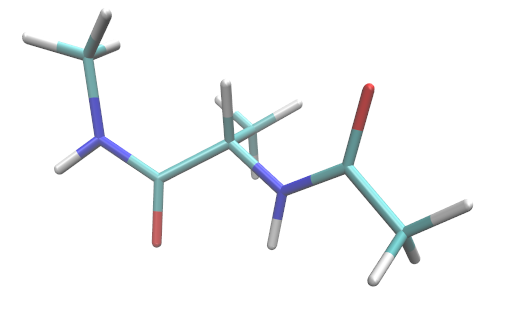
\includegraphics[width=10cm]{alanine.png}
\captionof{figure}{Alanine dipeptide, residues from left to right are NME, ALA and ACE}\label{fig:alanine}
\end{center}

\begin{center}
\begin{table*}[ht]
{
\hfill{}
\begin{tabular}{ c | c }
\hline 
 Parameter changed & Acceptance \%   \\  
\hline 
None & $<$ 3*$^1$ \\ 
\hline
Frozen bond LINCS & $<$ 5*$^1$ \\ 
\hline 
\end{tabular}}
\hfill{}
\caption{*$^1$simulations using standard classical parameters.  Acceptance when altering the classical potential for alanine dipeptide}
\label{table:alanine_altering_force_field}
\end{table*}
\end{center}

Although alanine dipeptide uses standard residues the acceptance is still very poor.  By freezing out the bond vibrations the acceptance slightly increases, however, this could just be an artefact of the stochastic nature of the method.

The next step was to freeze part of the system, initially this was selected to be the QM region, i.e. the ligand.  The ligand was allowed to move for the equilibration, then frozen and the water allowed to move around it.  The system selected was N$_2$ in 499 water and the acceptance was 13.2 \%.  If the ligand is allowed to move throughout the simulation, this acceptance drops to below 1 \%.  Although an improvement, this acceptance is still a little low.  Following this the water was frozen and the ligand allowed to move.  The results can be seen in table \ref{table:N2_frozen_water}.

\begin{center}
\begin{table*}[ht]
{
\hfill{}
\begin{tabular}{ c | c | c}
\hline 
 & Acceptance \% at $\lambda =1$ & Free Energy (kJ/mol)  \\  
\hline 
Run 1 & 39.8 & -487623.80 \\ 
\hline
Run 2 & 20.8 & -488176.35 \\ 
\hline 
\end{tabular}}
\hfill{}
\caption{Free energy and acceptance rate when allowing N$_2$ to move in frozen water}
\label{table:N2_frozen_water}
\end{table*}
\end{center}

A difference in the free energy of 552.55 kJ/mol for a simple system such as N$_2$ in water suggests major convergence problems.  If this method were to be applied to a more flexible ligand the results would be expected to show even worse convergence.



\section{Conclusions}

Using classical mechanics as a guiding potential to generate a QM/MM ensemble of structures in practice only works if the potential energy surfaces match.  The issue occurs within the acceptance criterion, as the acceptance depends on the energy difference between the potentials; if the energy difference is more negative it is accepted than the currently accepted snapshot.

The mismatch of the potential energy surfaces for ligands with low degrees of freedom is caused either by the interaction between the ligand and electrostatic embedded water or the intermolecular interaction in the solvent.  For larger ligands the number of degrees of freedom starts to have an effect on the acceptance.  

In order to improve acceptance in these cases, a bias could be applied to ensure that the structures with a large negative energy difference would not have such a large effect on the overall free energy.  This bias will be the focus of the next chapter.









